\subsection{}
\label{mandel:q:2}

\begin{quotation}
  \noindent
  \begin{enumerate}
  \item Compiler et exécuter le code original.
  \item Compiler et exécuter le code en changeant l'ensemble des
    paramètres.
  \item Commentez les résultats obtenus.
  \end{enumerate}
\end{quotation}

Pour compiler le code, on se place dans un environnement GNU, on
chemine dans le répertoire des sources, et on exécute la commande :

\begin{verbatim}
gcc -Wall -Wextra mandel.c \
  -o mandel -lm
\end{verbatim}

où la dernière option permet de lier la bibliothèque \texttt{math}.

Après exécution du programme, on obtient l'image de la figure
\ref{fig:default-image}.

\begin{figure}
  \centering
  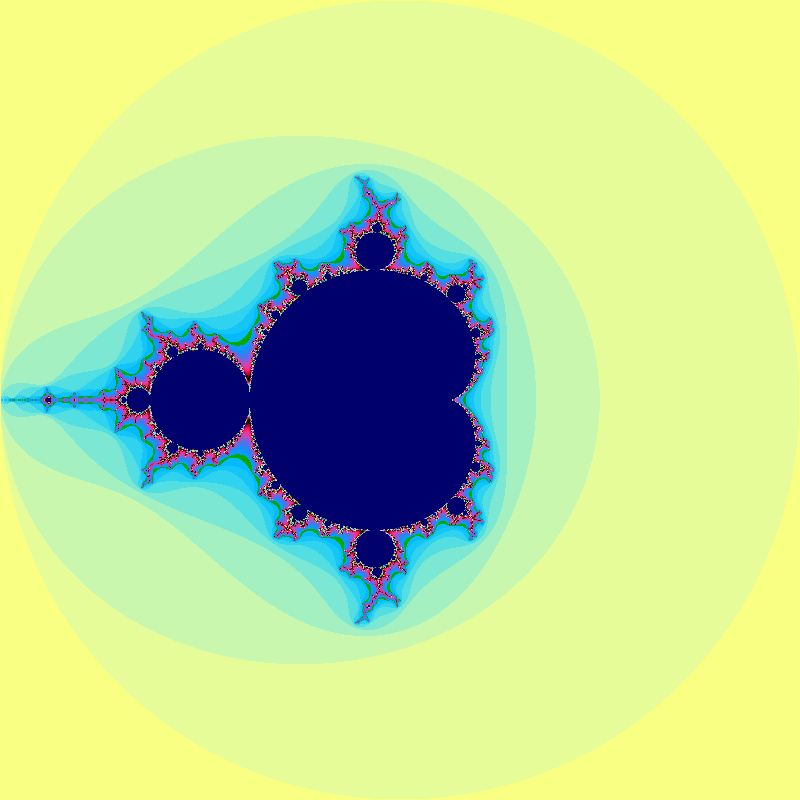
\includegraphics[width=0.8\linewidth]{../Resultats/800-10000}
  \caption{Fractale obtenue avec les paramètres par défaut}
  \label{fig:default-image}
\end{figure}

Le figure \ref{fig:mandel-seq-taille} montre l'évolution du temps de
calcul à une profondeur de 1000 en fonction de la taille d'un côté de
l'image demandée. Après une régression linéaire par moindres carrés,
on trouve les coefficients de la parabole $t = a x^2 + b x + c$
:\footnote{\textit{px} est une grandeur sans dimension !}


\[ \begin{cases}
    a = \num{3.1672e-07}  & s.px^{-2}\\
    b = \num{-6.5725e-05} & s.px^{-1}\\
    c = \num{3.7812e-02}  & s\end{cases} \]

\begin{figure}[t]
  \centering
  \begin{tikzpicture}
    \begin{axis}[
      xlabel={Côté de l'image (px)},
      ylabel={Temps de calcul (s)}
      ]
      \addplot table [x index=1, y index=4,
      col sep=semicolon, header=false]{\data/mandel-seq-taille.csv};
      
      \addplot+[no markers, samples=20, domain=0:2000] {3.1672e-7*x^2 - 6.5725e-5*x + 0.037812};
    \end{axis}
  \end{tikzpicture}

  \begin{tikzpicture}
    \begin{axis}[
      xlabel={Taille de l'image (px$^2$)},
      ylabel={Temps de calcul (s)}
      ]
      \addplot table [x expr=\thisrowno{1}^2, y index=4,
      col sep=semicolon, header=false]{\data/mandel-seq-taille.csv};
    \end{axis}
  \end{tikzpicture}

  \caption{Le temps de calcul est proportionnel au carré du côté de l'image.}
  \label{fig:mandel-seq-taille}
\end{figure}

En faisant varier la profondeur, on obtient la figure
\ref{fig:mandel-seq-prof}. On voit à nouveau que le temps de calcul
est proportionnel à la profondeur.

\begin{figure}
  \centering
  \begin{tikzpicture}
    \begin{axis}[
      xlabel={Profondeur},
      ylabel={Temps de calcul (s)}
      ]
      \addplot table [x index=3, y index=4,
      col sep=semicolon, header=false]{\data/mandel-seq-prof.csv};
    \end{axis}
  \end{tikzpicture}
  \caption{Le temps de calcul est proportionnel à la profondeur.}
  \label{fig:mandel-seq-prof}
\end{figure}

Dans le code, le calcul se fait au moyen de trois boucles \texttt{for}
imbriquées, dont la dernière réalise une opération en temps constant
(combinaison d'additions et de multiplications sur des entiers
processeurs). Les deux premières boucles itèrent sur chacun des côtés
de l'image, et la troisième sur la profondeur exigée. Ainsi, lorsque
la profondeur est fixée, la troisième boucle est une opération dont le
temps de calcul ne dépend pas de la taille de l'image ; cette
opération est faite autant de fois qu'il y a de pixels dans l'image,
ce qui explique la dépendance linéaire en fonction du nombre de pixels
observée à la figure \ref{fig:mandel-seq-taille}. Inversement, si la
taille de l'image est fixée, les deux boucles extérieures réalisent le
même nombre d'opérations ; puisque la troisième boucle réalise une
opération constante par niveau de profondeur, le temps de calcul
dépend linéairement du niveau de profondeur.

Pour une image 1000 $\times$ 1000, à un niveau de profondeur
\nombre{10000}, le temps de calcul est \nombre{2.815} secondes. Cette
valeur sera à comparer avec celles trouvées à la question \ref{mandel:q:4}.

%%% Local Variables:
%%% mode: latex
%%% TeX-master: "../rapport"
%%% End:
